%analysis body
%Created MS 05-11

\section{Analysis}\label{analysis}

\subsection{$^{85}$Rb and $^{87}$Rb Spin Analysis}\label{SpinAnalysis}

By measuring the resonant radiofrequencies used to induce the coupling of $m_F$ states, we can calculate the $g$-factors for $^{85}$Rb and $^{87}$Rb.  In Section \ref{MeasuringLinewidthandOpticalPumpingResonance}, we found the resonant frequencies to be $161.0 \pm 0.8$ kHz for $^{85}$Rb and $243.1\pm 0.3$ kHz for $^{87}$Rb.  (values for B, n, I?) Using Eqn. \ref{BLAH} we calculate $g_F$ for $^{85}$Rb to be $0.30\pm 0.03$ and $g_F$ for $^{87}$Rb to be $0.46\pm 0.05$.  Both calculations are in good agreement with the predicted values of $1/3$ and $1/2$ respectively. 

Using Eqn. \ref{eq:BLAH} and our calculated values for $g_F$, we can calculate the nuclear spins of both $^{85}$Rb and $^{87}$Rb in the $^{2}S_{1/2}$ atomic states.  Doing so, we calculate the nuclear spins to be $2.8 \pm 0.3$ and $1.7 \pm 0.2$ respectively.  These calculations are in good agreement with the predicted values of $5/2$ and $3/2$.  

The ratio of the measured $g-$factors between $^{87}$Rb and $^{85}$Rb is calculated to be $1.5 \pm 0.2$ as compared to the predicted value of $1/2$.  Finally the ratio of nuclear spins in the $^{2}S_{1/2}$ atomic state between $^{87}$Rb and $^{85}$Rb is calculated to be $0.61\pm 0.09$ as compared to the predicted value of $3/5$.  These ratios are in good agreement with theory.

Error in this measurement mostly arises due to the uncertainty in the magnetic field.  For both calculations, we assume that the magnetic field is produced by a perfect solenoid, namely $B=\mu_0 n I$.  Because the precision of our measurements of the center frequencies and solenoid current are very low (less than $1\%$), we suspect that this error is systematic due to the imperfection of the solenoid.  We estimate that this error to be approximately a factor of $10\%$. The presence of systematic error is supported by the relative accuracy of the ratios of the calculated $g-$factors and nuclear spins as compared to their absolute values.  

\subsection{Determination of $T_{1}$, $T_{2}$, and the Optical Pumping Time}\label{DeterminationofTimes}

To calculate the $T_1$ relaxation time, we use the data produced in Section \ref{MeasuringT1RelaxationandOpticalPumpingTime}.  To reconstruct the hidden exponential decay due to $T_1$ relaxation, we take several measurements similar to the sample data shown in Fig. \ref{fig:chop} for several different optical chopping frequencies.  We developed an algorithm in \emph{Mathematica} that would first measure the amount of dark time indicative of the chopping frequency used.  Following this measurement, the relative decrease in signal over the dark time was calculated by first fitting the subsequent rise due to optical pumping to an exponential curve.  This curve was then used to extrapolate the signal height at the end of the dark time (the time at which the laser light becomes unblocked and optical pumping begins).  This signal is then divided by the signal height immediately preceding the beginning of said dark time.  This relative signal height is then paired with the length of the dark time.  This process was repeated for over $40$ different chopping frequencies.  
\begin{figure}[htbp]
\begin{center}
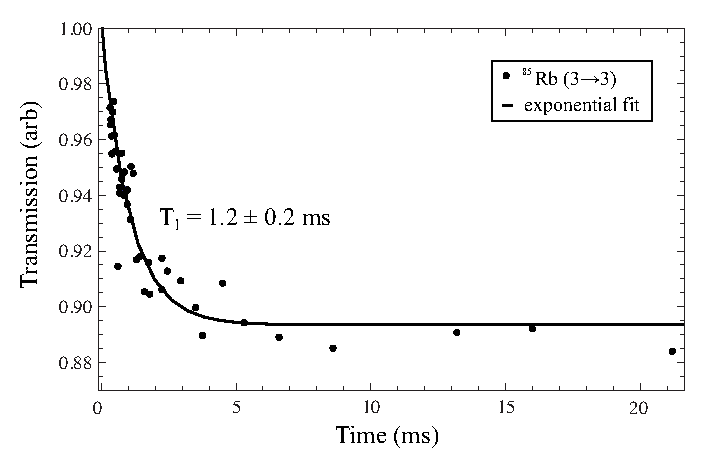
\includegraphics[height=70mm]{./figures/T1.eps}
\caption{\small{$T_1$ relaxation of $^{85}$Rb due to the blocking of laser light by an optical chopper.  This exponential decay was indirectly determined by measuring the relative decline in signal for different dark times as varied by the frequency of the optical chopper.  The $T_1$ relaxation time of this exponential decay is calculated to be $1.2\pm 0.2$ ms.}}
\label{fig:T1}
\end{center}
\end{figure}
Fig. \ref{fig:T1} shows the compiled data fit to an exponential decay.  This decay represents the hidden decay which we were unable to observe due to the blocking of laser light.  Using nonlinear regression analysis we calculate $T_1$ to be $1.2 \pm 0.2$ ms.  By fitting the exponential rise in signal due to optical pumping, we are also able use this algorithm to determine the optical pumping time $\tau$. We calculate $\tau=5.9 \pm 1.5$ ms.  

Error in both $T_1$ and $\tau$ mainly arises due to poor fitting by algorithm.  Any error in the fitting of the exponential rise due to optical pumping (the red curve in Fig. \ref{fig:chop}) greatly affects both values.  For this reason, it would be advantageous to fit the rise to as many data points as possible. Yet, due to the limited amount of data points, we are unable to consistently fit as well as we would like.  As a result, the statistical variation for $T_1$ values is quite large (shown by the distribution of points in Fig. \ref{fig:T1}). Likewise, the variation in $\tau$ is also quite large.  In order to combat this variation, data corresponding to short dark times (or high chopping frequencies) are removed.  At these frequencies, the decrease in signal due to $T_1$ relaxation is relatively low, thus the exponential rise due to optical pumping is also minimal.  The relative imprecision of fitting an exponential to a relatively flat distribution of data points forces us to exclude many of these points.


By measuring the natural linewidth of $^{85}$Rb , we can calculate the $T_2$ relaxation time.  In Section \ref{MeasuringLinewidthandOpticalPumpingResonance}, we found that the natural linewidth of $^{85}$Rb was $3.70 \pm 0.48$ kHz.  Using Eqn. \ref{eq:T2}, we calculate $T_2 = 86 \pm 12$ $\mu$s. The natural linewidth for $^{87}$Rb was calculated to be $5.35 \pm 0.47$ kHz, corresponding to a $T_2$ value of  $59 \pm 5$ $\mu$s.

Error in $T_2$ arises from error in the measurement of the linewidth. Part of this error comes from the algorithm used to calculate the linewidth.  Due to the difficulty in fitting the data to a lorentzian distribution, a more mechanical approach is taken to measure the linewidth. First the center frequency is found assuming  the data is symmetric. The highest data point below half-max is taken to half-max.  The difference between the frequencies corresponding to max and half-max is calculated and multiplied by two to give the linewidth (full width at half-max).  Accordingly error in this measurement is due to the step size between the points, which is $200$ Hz, and  any asymmetry of the resonance.  To minimize the the effect of asymmetry, resonances with low signal which typically exhibit asymmetry are excluded from the data. 

Error in the linewidth measurement is increased in the presence of any unchecked sources of power broadening or the existence of any magnetic field inhomogeneity within the magnetic field.  Any source of power broadening additional to RF field and laser light intensity would systematically increase our linewidth measurements causing our $T_2$ relaxation time to be artificially low.  More likely to distort our linewidth measurements, however, is the presence of inhomogeneous broadening discussed in Section \ref{BLAH}.  Inhomogeneities in the solenoid's uniform magnetic field would also systematically increase our linewidth measurement resulting in artificially low values for the $T_2$ relaxation time.  For example, a $5\%$ difference in magnetic field within the solenoid would correspond to broadening equal to $5\%$ the center frequency.  For $^{85}$Rb with a center frequency of $161.7$ kHz, broadening due to a $5\%$ inhomogeneity would be roughly $8\%$ kHz. We are unable to eliminate this source of systematic error.

Comparing the calculated values for $T_1$, $T_2$, and $\tau$, we see that $T_2$ is roughly an order of magnitude smaller.  This difference of magnitude could be indicative of additional broadening present during the the $T_2$ measurements such as power broadening due to the heater (which was shut off during the $T_1$ measurement).  However, if there are no systematic differences between the two measurements, the deviation in magnitude can be explained by the differences in the relaxation process.  Assuming that the data is correct, we predict that the time it takes for the pumped rubidium spin ensemble to deconhere is a roughly a factor of ten shorter than the lifetime of the pumped spin state of the rubidium atom. 


\subsection{Spin Exchange Analysis}\label{SpinExchangeAnalysis}

In Section \ref{MeasuringSpinExchange}, we found the spin exchange linewidths, $\gamma^{se}_2$ of $^{85}$Rb and $^{87}$Rb to be $2.80 \pm 0.28$ and kHz $3.92 \pm 0.71$ kHz respectively. Compared to the natural $\gamma_2$ linewidths $3.70 \pm 0.48$  kHz  and $5.35 \pm 0.47$ kHz, we see that our values for $\gamma^{se}_2$ are in agreement with Eqn. \ref{eqn:gamma2}.

By measuring the natural spin exchange linewidths of $^{85}$Rb and $^{87}$Rb, we are able to calculate the spin exchange time constant $T^{se}_2$.  Using Eqn. \ref{eq:Blah}, we determine $T^{se}_2$ to be $110 \pm 11$ $\mu$s for  $^{85}$Rb and $81 \pm 15$ $\mu$s for  $^{87}$Rb. 

Error in this spin exchange analysis arises due to the error in linewidth measurement.  This error is previously explained in Section \ref{DeterminationofTimes}.   We expect that the broadening due to inhomogeneities in the solenoid's magnetic field accounts for the presence of a systematic increase in $\gamma^{se}_2$ as we suspected for the systematic increase in $\gamma_2$.  Calculating the ratios of $\gamma^{se}_2$/$\gamma_2$ for $^{85}$Rb and $^{87}$Rb to be $0.76\pm 0.16$ and $0.73\pm 0.20$.  These ratios are comparable and thus support the claim that error in this calculation is systematic rather than statistical.